\documentclass{article}
\usepackage[hidelinks,bookmarks=false]{hyperref}
\usepackage{122}

\usepackage{graphicx}

\title{Биоинформатика \\ Домашнее задание №5}

\graphicspath{ {../bio/genotypes/} }

\begin{document}
  \maketitle

  \section{Выбранный человек} % Выбранная особь человека
  На сайте \url{https://opensnp.org/genotypes} есть много публичных генотипов,
  но, так как каждый из них был собран разными компаниями, у них встречаются разные форматы.
  Я выбрал формат AncestryDNA, потому что % Ксения тоже выбрал этот формат и я у него списываю
  там в самом начале файла есть большой коммент объясняющий специфику их формата,
  и потому что там сразу скачивается разархивированный файл
  и не надо пытаться заставить \texttt{gunzip} разархивировать файл без суффикса \texttt{.gz}.

  У меня получился человек \href{https://opensnp.org/users/10027}{\texttt{taylorsenestraro}} а данные скачиваются командой
  \texttt{curl -O \url{https://opensnp.org/data/10027.ancestry.8288}}

  \noindent
  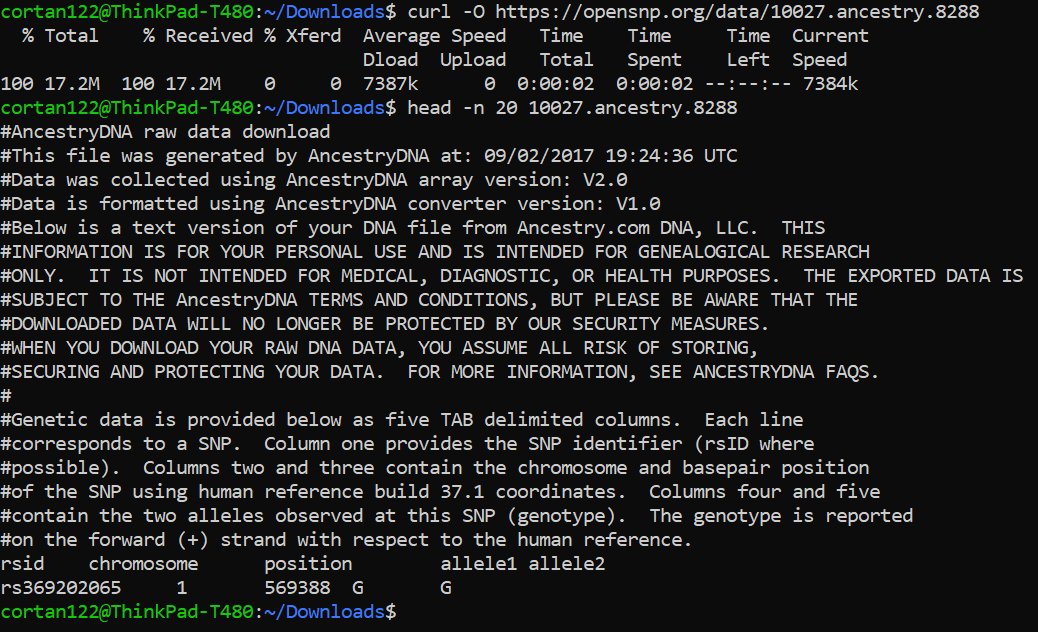
\includegraphics[width=\textwidth]{image20210313144544.png}

  Также у нас тут положительный strand и инвертировать алели не надо.

  \section{Цвет глаз}
  Для цвета глаз нам нужны
  \texttt{rs12913832}, \texttt{rs1800407}, \texttt{rs12896399}, \texttt{rs16891982}, \texttt{rs1393350} и \texttt{rs12203592}.

  \noindent
  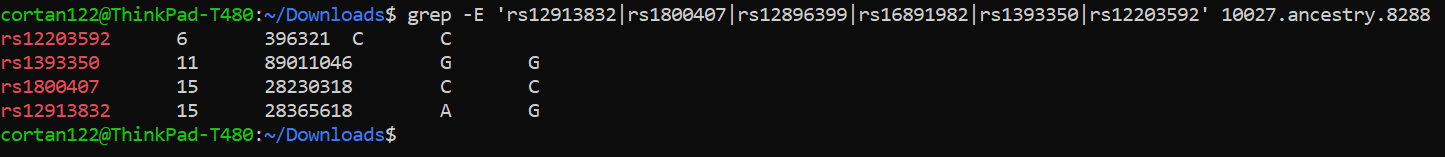
\includegraphics[width=\textwidth]{image20210313150216.png}

  Но rs12896399 и rs16891982 у нас нет, поэтому вводим NA, а rs12913832 инвертируем А в Т.

  \noindent
  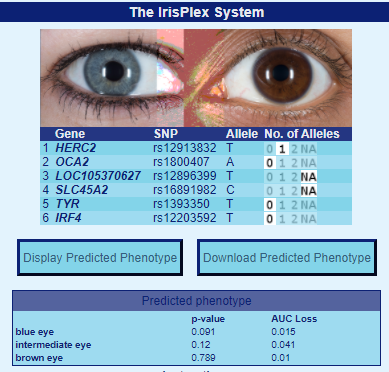
\includegraphics[width=\textwidth]{iris.png}

  Получается у нашего человека скорее всего голубые глаза.

  \section{Риск тромбоза}
  Тут нам нужны \texttt{rs6025}, \texttt{rs1799963}, \texttt{rs8176719}, \texttt{rs2066865} и \texttt{rs2036914}.

  \noindent
  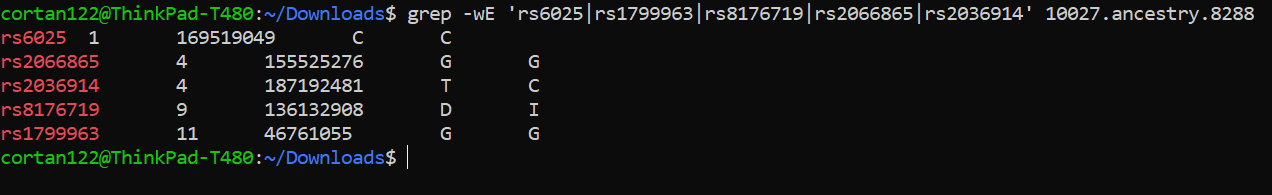
\includegraphics[width=\textwidth]{image20210313151316.png}

  \begin{center}
    \begin{tabular}{|l|l|l|l|}
      \hline
      \textbf{SNP} & \textbf{описание} & \textbf{у нас} & \textbf{риск в $n$ раз больше} \\
      \hline\hline
      \texttt{rs6025} & 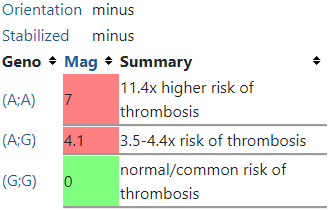
\includegraphics[width=5cm]{rs6025.png} & (G;G) & $1$ \\\hline
      \texttt{rs2066865} & 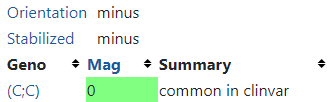
\includegraphics[width=5cm]{rs2066865.png} & (C;C) & $1$ \\\hline
      \texttt{rs2036914} & 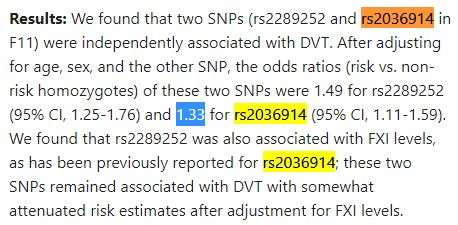
\includegraphics[width=5cm]{rs2036914.png} & (T;C) & $1.33$ \\\hline
      \texttt{rs8176719} & 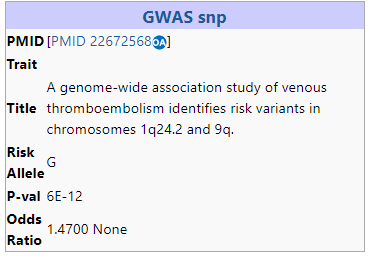
\includegraphics[width=5cm]{rs8176719.png} & (-;G) & $1.47$ \\\hline
      \texttt{rs1799963} & 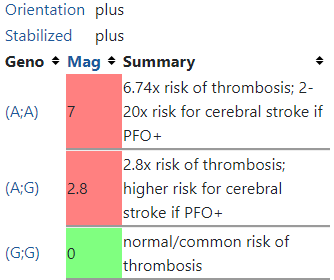
\includegraphics[width=5cm]{rs1799963.png} & (G;G) & $1$ \\\hline
    \end{tabular}
  \end{center}

  Риск получился в $1.33 \cdot 1.47 = 1.9551 \approx 2$ (два) раза больше.

  \section{Три рандомных снипа}
  У меня тут выбрались \texttt{rs4988235}, \texttt{rs9939609} и \texttt{rs1805007}.

  \noindent
  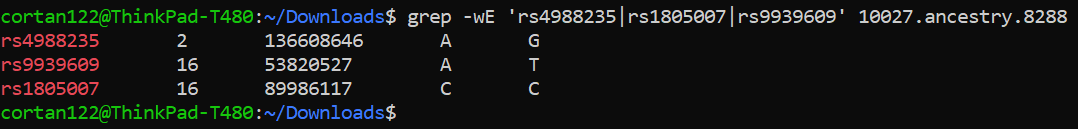
\includegraphics[width=\textwidth]{image20210313170346.png}

  \begin{center}
    \begin{tabular}{|l|l|l|l|}
      \hline
      \textbf{SNP} & \textbf{описание} & \textbf{у нас} & \textbf{вывод} \\
      \hline\hline
      \texttt{rs4988235} & 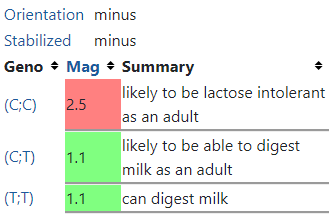
\includegraphics[width=5cm]{rs4988235.png} & (C;T) & скорее всего нету непереносимости лактозы \\\hline
      \texttt{rs9939609} & 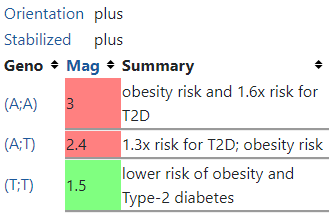
\includegraphics[width=5cm]{rs9939609.png} & (A;T) & в $1.3$ раза больше риска диабета и ожирения \\\hline
      \texttt{rs1805007} & 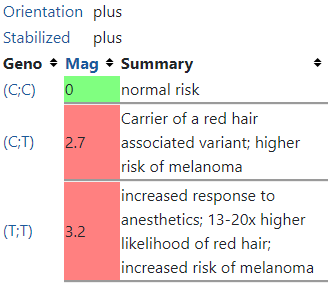
\includegraphics[width=5cm]{rs1805007.png} & (C;C) & всё норм \\\hline
    \end{tabular}
  \end{center}


\end{document}
